\chapter{Deriving Information from Data}
\chaplabel{information}

\section{Introduction}
This chapter introduces students to deriving useful information from raw data streams.

\section{Collecting Good Data}
Data collection is an important part of all of our lives. Everywhere we look, our eyes provide
us with data. Our ears and nose also provide lots of data to our brains. However, it is important
to realize why we might have a microcontroller collect data. Three reasons that come to mind are:
\begin{enumerate}
    \item Documentation - to record for posterity of some kind (e.g. world speed records)
    \item Actionable - do something based on the data (e.g. thermostat)
    \item Analysis - better understanding of our world (e.g. climate research)
\end{enumerate}

One big problem in life is to know whether the data we are collecting is good. Here are some
ways to check data to determine if it is worth looking at:
\begin{enumerate}
    \item Consistency
    \item Comparison to ground truth
    \item Repeatability
    \item Multiple sensors
    \item Common sense
\end{enumerate}

%\subsection{Consistency}

\subsection{Ground Truth}
One very good method of checking data is to compare to something that is more accurate than 
what you are using. For instance, if you are using a thermometer that is accurate to $\pm2^\circ$C,
compare it to a calibrated thermometer that is accurate to $\pm0.5^\circ$C. The calibration is 
important since it means that the more accurate thermometer has been tested against another
thermometer that is even more accurate that itself. Most test equipment needs regular calibration 
and gets a tag of some kind on it when it does get calibrated. Check that tag before using it.

\subsection{Repeatability}
If it is possible to repeat a data collection multiple times, comparing results will 
give some idea of whether the data is good. The standard deviation is one statistic that 
can give a useful estimate of how repeatable an experiment is. If the standard deviation is 
high (defining ``high" is important), than the data source probably is suspect.

\subsection{Multiple Sensors (sources)}
Another good way to check is to have multiple sources of the same information. If all three 
thermometers give the same result (within their error margins), then the data is more 
believable than just one thermometer. The shuttle ran with 5 computers with the general idea 
that there would be a vote between them in hopes that the majority would be correct. 
Sometimes it can be useful to have multiple sensors measuring the same thing but different ways. 
This can lead credence to the overall result. 

\subsection{Common Sense}
Lastly, it is important to check all measurements with a great deal of common sense. If it doesn't 
feel cold to you and the thermometer says it is 0~degrees, then you should suspect the thermometer 
is wrong. 

\subsection{Data Collection Review}
Check your data!
\begin{enumerate}
    \item How much do you trust your source?
    \item Does the data fit prior knowledge?
    \item Does it make sense? (Sanity check)
\end{enumerate}

\section{Sample Timing}
It is important to sample data at regular intervals. Jitter in sample timing can ruin the 
math of data analysis. The question is, how do we make sure that we are sampling at an 
even, regular interval? The simplest and most obvious method is shown in 
Listing~\ref{lst:wrongsampling}. This method might work for data that is sampled at a very 
slow rate--less than once a second. 

\begin{lstlisting}[language=C++, caption={This listing shows a simplistic way to time sampling.},label={lst:wrongsampling}]
void loop()
{
    static uint32_t currTime;
    currTime = millis();

    if(currTime - lastSampleTime >= sampleInterval) {
        doSampling();
        lastToggle = currTime;
    }
}
\end{lstlisting}

However, that the reality is more like what is shown in Listing~\ref{lst:simplesampleproblem}.
There are often processes running during the loop that introduce jitter into the sampling period.

\begin{lstlisting}[language=C++, caption={The problem with the simplistic approach is slow processes that introduce jitter.},label={lst:simplesampleproblem}]
void loop()
{
    static uint32_t currTime;
    currTime = millis();
    
    if(currTime - lastSampleTime >= sampleInterval) {
        doSampling();
        SOMETHING_SLOW();
        lastToggle = currTime;
    }
    SOMETHING_ELSE_OCCASIONALLY_SLOW();
}
\end{lstlisting}

So what is the solution? Interrupts!

\subsection{Interrupts}
Interrupts are as they sound: Normal code execution stops and the processor switches to a 
short piece of code called an Interrupt Service Routine (ISR or Interrupt Handler). Once 
the ISR finishes, code execution resumes where it had been interrupted. Interrupts can be 
triggered at specific repeatable times from onboard timers. They can also be triggered by 
other events. The thermometer on the board and the distance sensor can both be setup to 
trigger interrupts. 

ISRs must be short. They cannot even have \lstinline@Serial.println()@ calls inside them.
They typically do something like change a count, set a flag, toggle a value, start data 
collection (e.g. on an ADC), or read a value (e.g. also an ADC). If an ISR is too long 
regular code execution isn't resumed properly and the processor may reset and start over.
This can be triggered by a watchdog timer. 

\subsection{Volatile Variables}
It is important to designate any global variables that are changed by an ISR as 
\lstinline@volatile@. This designation tells the compiler not to optimize the variable 
out. This would normally happen since the compiler does not see the ISR called anywhere 
in the code. An example of doing this is shown in Listing~\ref{lst:volatile}

\begin{lstlisting}[language=C++, caption={This code illustrates using volatile for variables used in ISRs.},label={lst:volatile}]
volatile overtemp_flag = false;
void loop() {
    if(overtemp_flag) {
        overtemp_flag = false;
        // do something about being too warm
    }
}

interrupt void temp_isr() {
    overtemp_flag = true;
}
\end{lstlisting}

\section{Static Variables}
The second useful variable declaration when using interrupts (but is also useful elsewhere) is 
\lstinline@static@. The \lstinline@static@ declaration allows variables inside a function to 
persist between function calls, but keeps their scope inside the function. Listing~\ref{lst:staticvar}
demonstrates this with the variable named \lstinline@cnt@ inside the function \lstinline@count_int@. The
first time \lstinline@count_int@ is called \lstinline@cnt@ is initialized to a value of 0. Then it is 
incremented to 1. The second time \lstinline@count_int@ is called \lstinline@cnt@ has a value of 1 even 
though without the \lstinline@static@ declaration it would have a value of 0 every time the function was 
called. 

\begin{lstlisting}[language=C++, caption={This code demonstrates the functionality of a static variable.},label={lst:staticvar}]
int count_int() {
    static int cnt = 0;
    return(cnt++);
} 

void loop() {
    Serial.println(count_int());  // prints 0
    Serial.println(count_int());  // prints 1
}
\end{lstlisting}

\section{Extrema Detection}
I have found that I have often needed to find the peaks and valleys (the extrema) of a signal.
When working on a computer Python (scipy.signal.find\_peaks) and Matlab both have good algorithms
for peak (valley) detection. When working on a microcontroller there are also libraries
but it is important to understand what it is that you are looking for. Keep in mind that in 
an embedded (microcontroller) system we are usually processing data in real time and therefore 
need algorithms that work on live data coming in AND that do not take more processing power 
than is available between sample collections. Also, since the data is coming in continuously,
a simple maximum measurement or minimum will not work since we do not have all the data.

Some data has a flat baseline with only positive peaks as shown in Figure~\ref{fig:humidpeaks} of 
humidity sensor data. The temperature data shown in Figure~\ref{fig:temperaturepeaks} shows a drifting baseline and 
also positive peaks. Figure~\ref{fig:temphumidpeaks} shows temperature and humidity together for the same time
period. 

\begin{figure}[!htb]
	\centering
	\includegraphics[scale=0.4]{information/humidity.eps}
	\caption{Humidity measurements like this (with a human blowing on the sensor) demonstrate 
    positive peaks coming from a fairly stable baseline.}
	\label{fig:humidpeaks}
\end{figure}

\begin{figure}[!htb]
	\centering
	\includegraphics[scale=0.4]{information/Temperature.eps}
	\caption{Temperature measurements like this (with a human blowing on the sensor) demonstrate 
    positive peaks coming from a drifting baseline.}
	\label{fig:temperaturepeaks}
\end{figure}

\begin{figure}[!htb]
	\centering
	\includegraphics[scale=0.4]{information/TempHum.eps}
	\caption{This shows both temperature and humidity on the same graph. Notice the different intensity
    of peaks between the two for the same events and teh difference in times for the peaks for the 
    same events.}
	\label{fig:temphumidpeaks}
\end{figure}

Other data has a baseline with positive and negative deviations such as the accelerometer data 
shown in Figure~\ref{fig:accelpeaks} Some algorithms are better for one or the other or may work for both situations.

\begin{figure}[!htb]
	\centering
	\includegraphics[scale=0.4]{information/rawAccel.eps}
	\caption{This accelerometer data demonstrates both positive and negative peaks from a baseline.}
	\label{fig:accelpeaks}
\end{figure}

The data so far has had pretty quiet baselines. Oftentimes, data can be much noisier as is illustrated 
in the light sensor data shown in Figure~\ref{fig:lightpeaks}.

\begin{figure}[!htb]
	\centering
	\includegraphics[scale=0.4]{information/light.eps}
	\caption{This light sensor (CDS cell into ADC) is noisy as sensor data can often be.}
	\label{fig:lightpeaks}
\end{figure}

\subsection{Thresholding}
The simplest algorithm is a simple threshold system. This is used in most thermostats. It is measuring
the temperature and if it gets above the threshold, it turns on the air conditioning. The threshold 
is now switched to a lower value (to prevent oscillations) and it now looks for the temperature to 
drop below the threshold. The first threshold required a positive derivative. The second threshold 
required a negative derivative. These are important distinctions. 

Thresholding is simple to implement and can be useful in many situations. Obstacle detection is another 
example where we only care if the object is closer than some threshold. An example of a simple threshold
valley detection is shown in Figure~\ref{fig:lightthresh}. Note that this method gives lots of points
for each valley.

\begin{figure}[!htb]
	\centering
	\includegraphics[scale=0.4]{information/light-thresh.eps}
	\caption{Looking for light values less than a threshold of 200 gives many points for each valley
    in this data.}
	\label{fig:lightthresh}
\end{figure}

There is one more type of situation to think about. The potentiometer data shown in 
Figure~\ref{fig:potvalues} is an example where the baseline of the data shifts after an event.

\begin{figure}[!htb]
	\centering
	\includegraphics[scale=0.4]{information/pot.eps}
	\caption{This potentiometer data shows the situation where the baseline shifts after 
    an extrema event.}
	\label{fig:potvalues}
\end{figure}

\subsection{Dispersion Method}
To understand this version of extrema detection (and some others) a bit of terminology needs to 
be understood. The first is the baseline of a signal. \href{https://bmcbioinformatics.biomedcentral.com/articles/10.1186/1471-2105-10-4/figures/2}
{This figure} shows a signal that has a decreasing baseline. The baseline can be thought of as where the 
signal is when no extrema is present. It is often measured by some sort of low pass filter such as a moving 
average. 

Once we determine the baseline of a signal, we can look for divergences from the baseline. One way to 
measure that divergence is to measure how many standard deviations away from the baseline a particular 
point lands. We can then set a threshold of how many standard deviations away from the baseline is 
considered an extrema.

For the dispersion/z-score method, the last parameter to look at is the influence which is a value 
between 0 and 1. An influence of 0 means that points that are considered extrema are not used in 
calculating the baseline. This does assume that the mean and standard deviation of the signal do 
not change over time. Since that is rarely, the case it is best to set the influence to something greater 
than 0. An influence of 1 means that extrema points influence the mean and standard deviation the 
same as all the other points. That is also rarely a good idea since averages are particularly sensitive
to outliers and by definition, the extrema are outliers. A median filter or a 
\href{https://en.wikipedia.org/wiki/Exponential\_smoothing}{simple exponential filter} might work better
for some situations.

As with all algorithms, the parameters will have to be chosen and tuned to work with the particular data 
you are measuring.

\section{Bayes Theorem}
A pattern classifier can be thought of as a set of functions, $g_i(\bar{x})$, called discriminant 
functions. There is a discriminant function for each class, $\omega_i$, that evaluates a particular 
set of data, $\bar{x}$. The classification rule is then: 

\noindent Assign $\bar{x}$ to class $\omega_i$ if 
\begin{equation}
    g_i(\bar{x}) > g_j(\bar{x})\ \mathrm{for\ all}\ j \neq i
\end{equation}

A good and helpful option to explore for $g_i$ is called Bayes Theorem. The formula for Bayes Theorem
is shown in Equation~\ref{eq:bayes}. 

\begin{equation} \label{eq:bayes}
    P\left(\omega_i | \bar{x}\right) = \frac{p(\bar{x}|\omega_i)P(\omega_i)}{p(\bar{x})}
\end{equation}

where
\begin{itemize}
    \item $\bar{x}$ is the data. If we are classifying faces is an image of a face 
    \item $\omega_i$ is class $i$, one of the possible identities of the face we are trying to classify 
    \item $P(\omega_i|\bar{x})$ is the posterior probability--the probability of $\omega_i$ 
            given $\bar{x}$. In the example, it is the probability that the 
            face image belongs to me rather than someone else in the database.
    \item $p(\bar{x}|\omega_i)$ is the likelihood or state conditional probability density function. 
            This is the probability that $\bar{x}$ occurred given class $\omega_i$. For example what 
            is the probability of that the face image given that it is of me. The likelihood is 
            calculated based on collected data.
    \item $P(\omega_i)$ is the prior probability of class $\omega_i$. Rolling a single 6~sided die gives 
            equal probability of each number so the priors are all $1/6$. However, if instead we look at 
            the sum of rolling 2 dice the probabilities of each number is no longer the same and the 
            priors are different. The priors are calculated from existing, collected data.
    \item $p(\bar{x})$ is the evidence which is a scale factor to keep the probabilities summing to 1
    \begin{equation}
        \sum_j P(\omega_j|\bar{x}) = 1
    \end{equation}
            The evidence is calculated from existing, collected data as
    \begin{equation}
        p(\bar{x}) = \sum_j p(\bar{x}|\omega_j)P(\omega_j)
    \end{equation}
\end{itemize}

Discriminant functions are not unique. As long as $f(\cdot)$ is monotonically increasing 
$f(g_i(\bar{x}))$ will work too. Therefore, all of the Equations~\ref{eq:discriminants} will work.

\begin{subequations}
    \label{eq:discriminants}
    \begin{align}
        g_i(\hat{x}) =& P(\omega_i|\bar{x}) \\
                     =& \frac{p(\hat{x}|\omega_i)P(\omega_i)}{\sum_j p(\hat{x}|\omega_j)P(\omega_j)} \\
                     =& p(\hat{x}|\omega_i)P(\omega_i) \\
                     =& \ln\left(p\left(\hat{x}|\omega_i\right)\right) + \ln\left(P\left(\omega_i\right)\right)
    \end{align}
\end{subequations}

\section{ML Metrics}

\subsection{Confusion Matrix}
\begin{table}[!ht]
	\centering
	\begin{tabular}{c c | c c c | c}
        & & \multicolumn{3}{c|}{Predicted} & \\
         & & A & B & C & Total \\
        \hline
        \multirow{3}{*}{\rotatebox[origin=c]{90}{Actual}} & A & 10 & 1 & 2 & 13 \\
        & B & 3 & 11 & 4 & 18 \\
        & C & 5 & 6 & 12 & 23 \\
        \hline
        & Total  & 18 & 18 & 18 & 54
	\end{tabular}
	\caption{This shows what the rows and columns of a confusion matrix mean.}
	\label{table:confusionmatrix}
\end{table}

\begin{equation}
    \begin{bmatrix}
        10 & 1 & 2 \\
        3 & 11 & 4 \\
        5 & 6 & 12
    \end{bmatrix}
\end{equation}

\subsection{Accuracy}
\begin{equation}
    \mathrm{Accuracy} = \frac{\mathrm{\# correct}}{\mathrm{\# predictions}}
    = \frac{10+11+12}{1+2+3+4+5+6+10+11+12} = 0.61
\end{equation}


\subsection{Precision}
Precision is only calculated per class. Overall precision ends up as the
same as overall accuracy. Precision can be thought of as accuracy by column
of a confusion matrix. 
\begin{equation}
    \mathrm{Precision} = \frac{\mathrm{\# True Positives}}{\mathrm{\# True Positives}+\mathrm{\# False Positives}}
\end{equation}
For class A in the example (Table \ref{table:confusionmatrix}), the precision
would be:
\begin{equation}
    \mathrm{PrecA}=\frac{10}{10+3+5} = 0.56
\end{equation}

\subsection{Recall}
Recall is also only calculated per class because calculating it for everything
also degenerates to overall accuracy. Recall can be thought of as looking 
along the rows of the confusion matrix.
\begin{equation}
    \mathrm{Recall} = \frac{\mathrm{\# True Positives}}{\mathrm{\# True Positives}+\mathrm{\# False Negatives}}
\end{equation}
For class A in the example (Table \ref{table:confusionmatrix}), the recall
would be:
\begin{equation}
    \mathrm{RecallA}=\frac{10}{10+1+2} = 0.77
\end{equation}


\subsection{F1 Score}
F1 score is the harmonic mean of precision and recall and therefore is also 
only calculated on a per class basis.
\begin{equation}
    \mathrm{F1 Score} = 2*\frac{\mathrm{Precision*Recall}}{\mathrm{Precision+Recall}}
\end{equation}
For class A in the example (Table \ref{table:confusionmatrix}), the F1 score
would be:
\begin{equation}
    \mathrm{F1A}=2\left(\frac{0.56 * 0.77}{0.56+0.77}\right) = 0.65
\end{equation}



\subsection{References}
\begin{enumerate}
    \item \href{https://stackoverflow.com/questions/22583391/peak-signal-detection-in-realtime-timeseries-data}
                {This is a very good discussion of real-time peak detection algorithms and examples}
    \item \href{https://bmcbioinformatics.biomedcentral.com/articles/10.1186/1471-2105-10-4}
                {https://bmcbioinformatics.biomedcentral.com/articles/10.1186/1471-2105-10-4}
    \item \href{https://forum.arduino.cc/t/detection-of-a-vibration-peak/423080/9}{Very simple peak detector} that just
                looks for points above a threshold
    \item \href{https://github.com/leandcesar/PeakDetection}{An Arduino library for dispersion method}
\end{enumerate}
